% based on Model 3 of Activity 12 - Internet by Helen Hu

\model{How the Internet Works}

All devices connected to the Internet are assigned an \emph{IP address} made up of four 8-bit numbers separated by dots (e.g., 173.194.208.139). Some are assigned a \emph{static} (permanent) IP address, whereas others are assigned a \emph{dynamic} (temporary) IP address. Since it's difficult for people to remember numbers, we typically use \emph{domain names} when referring to websites.

\begin{center}
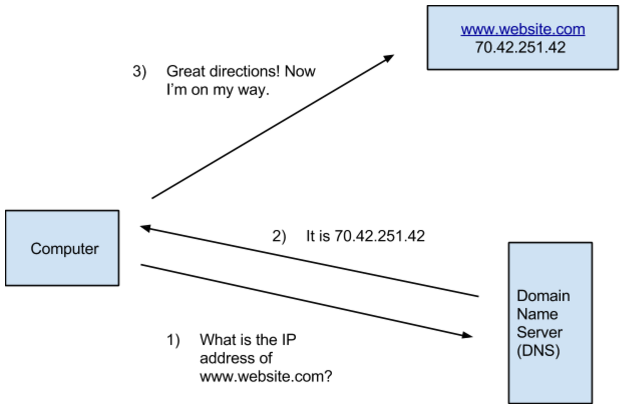
\includegraphics[width=0.75\textwidth]{CSP/dns1.png}
\end{center}


\quest{15 min}


\Q Based on the paragraph above:
\begin{enumerate}
\item How many bits does an IP address have? \ans{32 bits}
\item What is the largest possible IP address? \ans{255.255.255.255}
\end{enumerate}


\Q Based on the diagram above:
\begin{enumerate}
\item What is the domain name of the requested server? \ans{www.website.com}
\item What is the IP address of the requested server? \ans{70.42.251.42}
%\item What is the binary version of the IP address in the above model?
\end{enumerate}


\Q In your own words, what is the function of a DNS server?

\begin{answer}
It translates domain names into IP addresses upon request.
DNS maintains a database of all registered domain names.
\end{answer}


\Q Give examples of domain names that you use frequently.
Name at least two .com, two .org, two .edu, and two of something else.

% see https://domaintyper.com/top-websites/
\begin{answer}[5em]
Examples may include:
google.com, facebook.com, youtube.com;
wikipedia.org, craigslist.org, wordpress.org;
mit.edu, stanford.edu, harvard.edu;
sourceforge.net, irs.gov, bit.ly
\end{answer}


\Q How are domain names an example of an abstraction?

\begin{answer}[5em]
They represent an IP address; it's much easier to remember a name than four specific numbers.
Also the suffix (.com, .org. edu) indicates what type of domain it is (e.g., commercial, organization, educational).
\end{answer}


\Q List the IP addresses for two of your lab computers and two of your phones.
(You can search Google for ``IP address'' to find them.)

\begin{answer}[5em]
Answers will vary depending on the student's location.
\end{answer}


\Q Go to \href{http://www.tcpiputils.com/}{TCPIPutils.com} and search for your school's domain name.
Scroll down half-way to ``Network information''.
\begin{enumerate}
\item Identify the range of IP addresses used by your school. \ans{134.126.0.0 -- 134.126.255.255}
\item Does the university have enough IP addresses for all students, faculty, and staff (and their multiple devices)? Explain your answer.
\end{enumerate}

\vspace{-1em}

% see https://www.jmu.edu/about/fact-and-figures.shtml
\begin{answer}[5em]
JMU has about 21,000 students plus 1,500 faculty and staff.
With a 16-bit range, there are $2^{16} = 65,536$ possible IP addresses.
That means we have about 2.9 IP addresses per person.
But some of the addresses are for computer labs, campus servers, etc.
And it's not uncommon for people to have both a computer and a phone.
At some point, we're going to run out of IP addresses.
\end{answer}
